\documentclass[tikz]{standalone}
\usepackage{tikz}
\usepackage{xcolor}

% Eigene Farben definiert (nun optimiert für hellen Hintergrund)
\definecolor{rot}{RGB}{204,0,0}
\definecolor{blau}{RGB}{0,102,204}
\definecolor{orange}{RGB}{204,85,0}
\definecolor{gruen}{RGB}{0,153,0}
\definecolor{dunkelgruen}{RGB}{0,153,0}
\definecolor{dunkelblau}{RGB}{0,128,128}
\definecolor{backcolor}{RGB}{235,245,255}
\definecolor{frontcolor}{RGB}{220,220,220}
\definecolor{hellblau}{RGB}{180,210,235}
\definecolor{lila}{RGB}{153,0,153}
\definecolor{gelb}{RGB}{204,153,0}
\definecolor{dunkelrot}{RGB}{153,0,51}
\definecolor{dunkelgelb}{RGB}{153,153,0}

\newcommand{\rot}[2][rot]{\textcolor{#1}{#2}}
\newcommand{\gruen}[2][gruen]{\textcolor{#1}{#2}}
\newcommand{\frontcolor}[2][frontcolor]{\textcolor{#1}{#2}}
\newcommand{\gelb}[2][gelb]{\textcolor{#1}{#2}}
\newcommand{\orange}[2][orange]{\textcolor{#1}{#2}}
\newcommand{\blau}[2][blau]{\textcolor{#1}{#2}}
\newcommand{\hellblau}[2][hellblau]{\textcolor{#1}{#2}}
\newcommand{\lila}[2][lila]{\textcolor{#1}{#2}}
\newcommand{\dunkelrot}[2][dunkelrot]{\textcolor{#1}{#2}}
\newcommand{\dunkelgelb}[2][dunkelgelb]{\textcolor{#1}{#2}}


\begin{document}
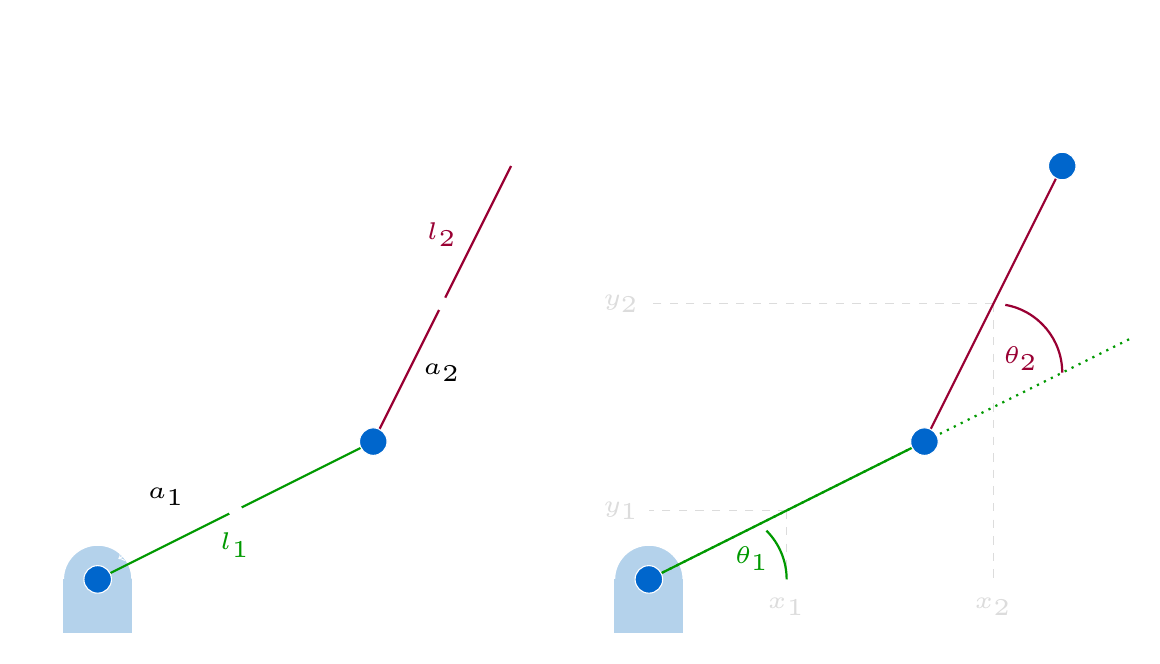
\begin{tikzpicture}[scale = 1.75, every node/.style={transform shape}]
    % Koordinatensystem
    %\draw[very thin, gray] (-5,-5) grid (5,5); % Raster
    %\draw[->] (-5,0) -- (5,0); % x-Achse
    %\draw[->] (0,-5) -- (0,5); % y-Achse
    
    % Achsen und Hilfslinien
    \draw[white, dashed, ->] (0.0,-1.0) -- (3.5,-1.0);
    \draw[white, dashed, ->] (0.0,-1.0) -- (0.0,3.0);
    
    % Schwerpunkte
    \draw[frontcolor, dashed] (1.0,-0.5) -- (1.0,-1.0);
    \draw[frontcolor, dashed] (1.0,-0.5) -- (0,-0.5);
    \node at (-0.2, -0.5) {\tiny $\frontcolor{y_1}$};  % Punktbeschriftung
    \node at (1, -1.2) {\tiny $\frontcolor{x_1}$}; 
    \draw[frontcolor, dashed] (2.5,1) -- (0.0,1);
    \draw[frontcolor, dashed] (2.5,1) -- (2.5,-1);
    \node at (-0.2, 1.0) {\tiny $\frontcolor{y_2}$};  % Punktbeschriftung
    \node at (2.5, -1.2) {\tiny $\frontcolor{x_2}$}; 

    % Erste Zeichnung (Original)
    \fill[hellblau] (-4,-1) circle (0.25);  % Füllt das Objekt mit hellblau
    \draw[white, line width = 0.2mm] (-4,-1) circle (0.25);  % Weißer Rand um das Objekt
    
    \draw[white, line width = 0.2mm] (-4.25,-1.4) rectangle (-3.75,-1);  % Weißer Rand um das Rechteck
    \fill[hellblau] (-4.25,-1.4) rectangle (-3.75,-1);  % Füllt das Rechteck mit hellblau
    \draw[thick, white] (-4.5,-1.4) -- (-3.5,-1.4);
    
    % Grüne Linie angepasst (Endpunkt auf (-2.0, 0.0))
    \draw[thick, gruen] (-4,-1) -- (-2.0,0.0);
    
    % Rote Linie angepasst (von (-2.0, 0.0) nach (-1.0, 2.0))
    \draw[thick, dunkelrot] (-2.0,0.0) -- (-1.0,2.0);
    
    % Glieder
    \fill[blau] (-2.0,0.0) circle (0.1);
    \draw[white, thin] (-2.0,0.0) circle (0.1);  % Weißer Rand um das Objekt
    \fill[blau] (-4.0,-1.0) circle (0.1);
    \draw[white, thin] (-4.0,-1.0) circle (0.1);  % Weißer Rand um das Objekt
    
	% Beschriftungen
	\node at (-3, -0.75) {\tiny $\gruen{l_1}$};  % 
	\node at (-1.5, 1.5) {\tiny $\dunkelrot{l_2}$};  % 
	
	% Schwerpunkte 
	\fill[white] (-3.0,-0.5) circle (0.05);
	\fill[white] (-1.5,1) circle (0.05);
	
	\draw[white, <->] (-1.85,0.15) -- (-1.5,0.85);
	\draw[white, <->] (-3.85,-0.85) -- (-3.1,-0.45);
	
	% Beschriftungen
	\node at (-3.5, -0.4) {\tiny $a_1$};  % 
	\node at (-1.5, 0.5) {\tiny $a_2$};  % 
    
    % Zweite Zeichnung (verschoben um 4 Einheiten entlang der x-Achse)
    \fill[hellblau] (0,-1) circle (0.25);  % Füllt das Objekt mit hellblau
    \draw[white, line width = 0.2mm] (0,-1) circle (0.25);  % Weißer Rand um das Objekt
    
    \draw[white, line width = 0.2mm] (-0.25,-1.4) rectangle (0.25,-1);  % Weißer Rand um das Rechteck
    \fill[hellblau] (-0.25,-1.4) rectangle (0.25,-1);  % Füllt das Rechteck mit hellblau
    \draw[thick, white] (-0.5,-1.4) -- (0.5,-1.4);
    
    % Grüne Linie (verschoben)
    \draw[thick, gruen] (0,-1) -- (2.0,0.0);
    \draw[thick, gruen, dotted] (0,-1) -- (3.5,0.75);
    
    % Rote Linie (verschoben)
    \draw[thick, dunkelrot] (2.0,0.0) -- (3.0,2.0);
    
    % Glieder
    \fill[blau] (2.0,0.0) circle (0.1);
    \draw[white, thin] (2.0,0.0) circle (0.1);  % Weißer Rand um das Objekt
    \fill[blau] (0.0,-1.0) circle (0.1);
    \draw[white, thin] (0.0,-1.0) circle (0.1);  % Weißer Rand um das Objekt
    \fill[blau] (3.0,2.0) circle (0.1);
    \draw[white, thin] (3.0,2.0) circle (0.1);  % Weißer Rand um das Objekt
    
    % Winkel
    \draw [gruen, thick] (1,-1)  arc[start angle=0,end angle=45,radius=0.5cm];
	\node at (0.75, -0.85) {\tiny $\gruen{\theta_1}$};  % Winkelbeschriftung
	
	\draw [dunkelrot, thick] (3,0.5)  arc[start angle=0,end angle=80,radius=0.5cm];
	\node at (2.7, 0.6) {\tiny $\dunkelrot{\theta_2}$};  % Winkelbeschriftung
\end{tikzpicture}
\end{document}
